\section{REST-API}
	Der Server hat die Aufgabe den Client zur Verfügung zu stellen
	und einige Funktionen mittels einer REST-Schnittstelle zur Verfügung zu stellen, dem API.
	Das API ist RESTful auf dem Level 2\footnote{REST Maturity Model: \url{http://de.wikipedia.org/wiki/Representational\_State\_Transfer\#REST\_Maturity\_Model}}.
	Das heisst, die einzelnen Elemente haben ihre eigenen Adressen
	und können mit den HTTP-Verben "'GET"', "'POST"' und "'DELETE"' verwendet werden.
	
	Sowohl für die Entwicklung des Clients wie auch für die weitere Entwicklung von \eeppi\ wurde das API des Servers dokumentiert.
	Ein Ausschnitt der API Dokumentation ist in Abbildung\ \ref{fig:apiScreenshot} abgebildet.
	Das Konzept und die Methodik der Dokumentation wurde als Teil von \eeppi\ erstellt
	und ist strukturell an das API von Jira\footnote{\url{https://docs.atlassian.com/jira/REST/latest/}} angelehnt.
	Damit das API mit möglichst geringem Aufwand auf dem neusten Stand bleibt, wurde darauf geachtet,
	die darin angezeigten Daten möglichst direkt aus den Originalquellen zu beziehen oder zumindest möglichst nah davon.
	
	\subsection{Herkunft der Daten}
		\subsubsection{Liste aller API-Methoden}
			Die Liste aller Methoden wird direkt aus den Programmcode abgeleitet.
			Dazu wird mit Hilfe von Reflections\footnote{\url{http://docs.oracle.com/javase/7/docs/api/java/lang/reflect/package-summary.html}} in einem ersten Schritt die Liste aller Controller-Klassen eruiert
			und in einem zweiten Schritt von diesen die Methoden extrahiert, die einen API-Aufruf repräsentieren.
		
		\subsubsection{HTTP-Verb und Pfad}
			Das HTTP-Verb und der Pfad, mit welchem die Methode aufgerufen werden kann,
			werden aus der "'routes"'-Datei geladen.
			Auch das Serverframework (Play Framework) lädt diese Informationen aus dieser Datei,
			wenn es Anfragen von Clients an den richtigen Controller delegieren will.
			
		\subsubsection{Beschreibungen}
			Die verschiedenen Beschreibungen für die Methoden werden aus Annotationen direkt bei der Controller-Methode generiert.
			In Abbildung\ \ref{fig:apiAnnotations} ist ein Beispiel eines Controllers mit Annotationen abgebildet.
			Die Annotationen beschreiben:
			\begin{itemize}
				\item{alle Parameter}
				\item{die Methode im Ganzen}
				\item{alle möglichen Rückgabe-Stati und deren konkrete Bedeutung}
				\item{ob eine Authentifizierung nötig ist}
				\item{die Beispielaufrufe (siehe \ref{subsubsec:exampleQueries})}
			\end{itemize}
			\begin{figure}[H]
				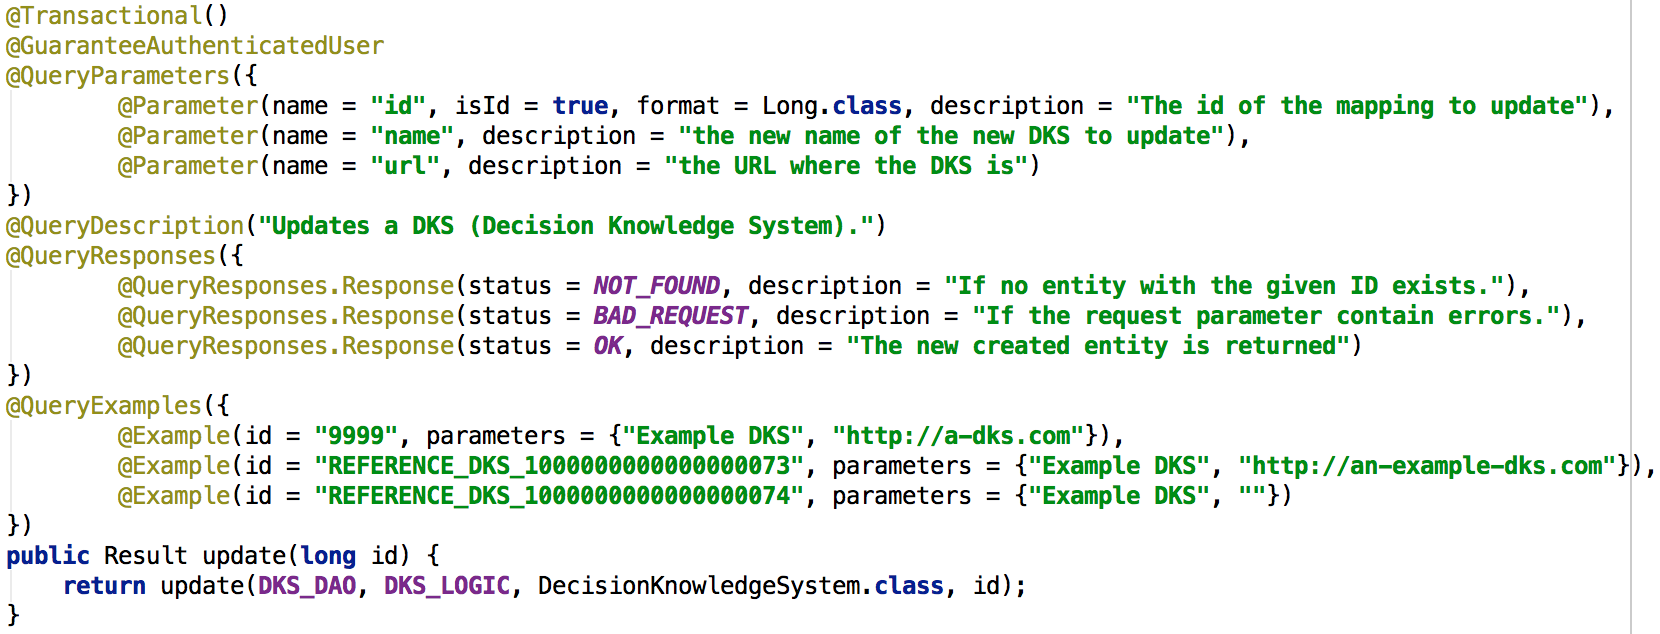
\includegraphics[width=0.9\textwidth]{codeDocumentation/media/img/apiAnnotations.png}
				\centering
				\caption{Annotations im DecisionKnowledgeSystemController}
				\label{fig:apiAnnotations}
			\end{figure}
			
	\subsection{Beispielaufrufe}
	\label{subsubsec:exampleQueries}
		Um dem Benutzer garantieren zu können, dass und wie die Methode wirklich funktioniert,
		werden für jede Methode Beispielaufrufe und deren Antworten live generiert und angezeigt.
		Dazu werden bei jeder Generierung der API Dokumentation zuerst einige Beispieldaten erstellt
		und anschliessend auf diesen Daten die Methode wie ein externer, unabhängiger Client aufgerufen.
		Die erhaltenen Ergebnisse werden dann in der API als "'The previous command \textbf{did} return"' angezeigt.
		Falls eine solche Simulation, beispielsweise aufgrund von externen Abhängigkeiten, nicht möglich ist,
		so ist die vom Entwickler erwartete Antwort auch in der Annotation definiert und wird dem Benutzer als
		"'The previous command \textbf{would probably} return"' angezeigt.
		
		Damit die dafür generierten Beispieldaten nicht mit den echten Daten des Systems interferieren,
		existiert für diesen Teil eine separate Datenbank.
		Diese muss der Benutzer jedoch nicht konfigurieren.
		Da die Daten nur während der Generation der API Dokumentation benötigt werden
		und nicht längerfristig persistiert werden müssen,
		werden sie lediglich in einer SQLite-Datenbank\footnote{Einfache Datenbank, in welcher die Daten in einer einzigen Datei gespeichert werden} gespeichert.
	
	\begin{figure}[H]
		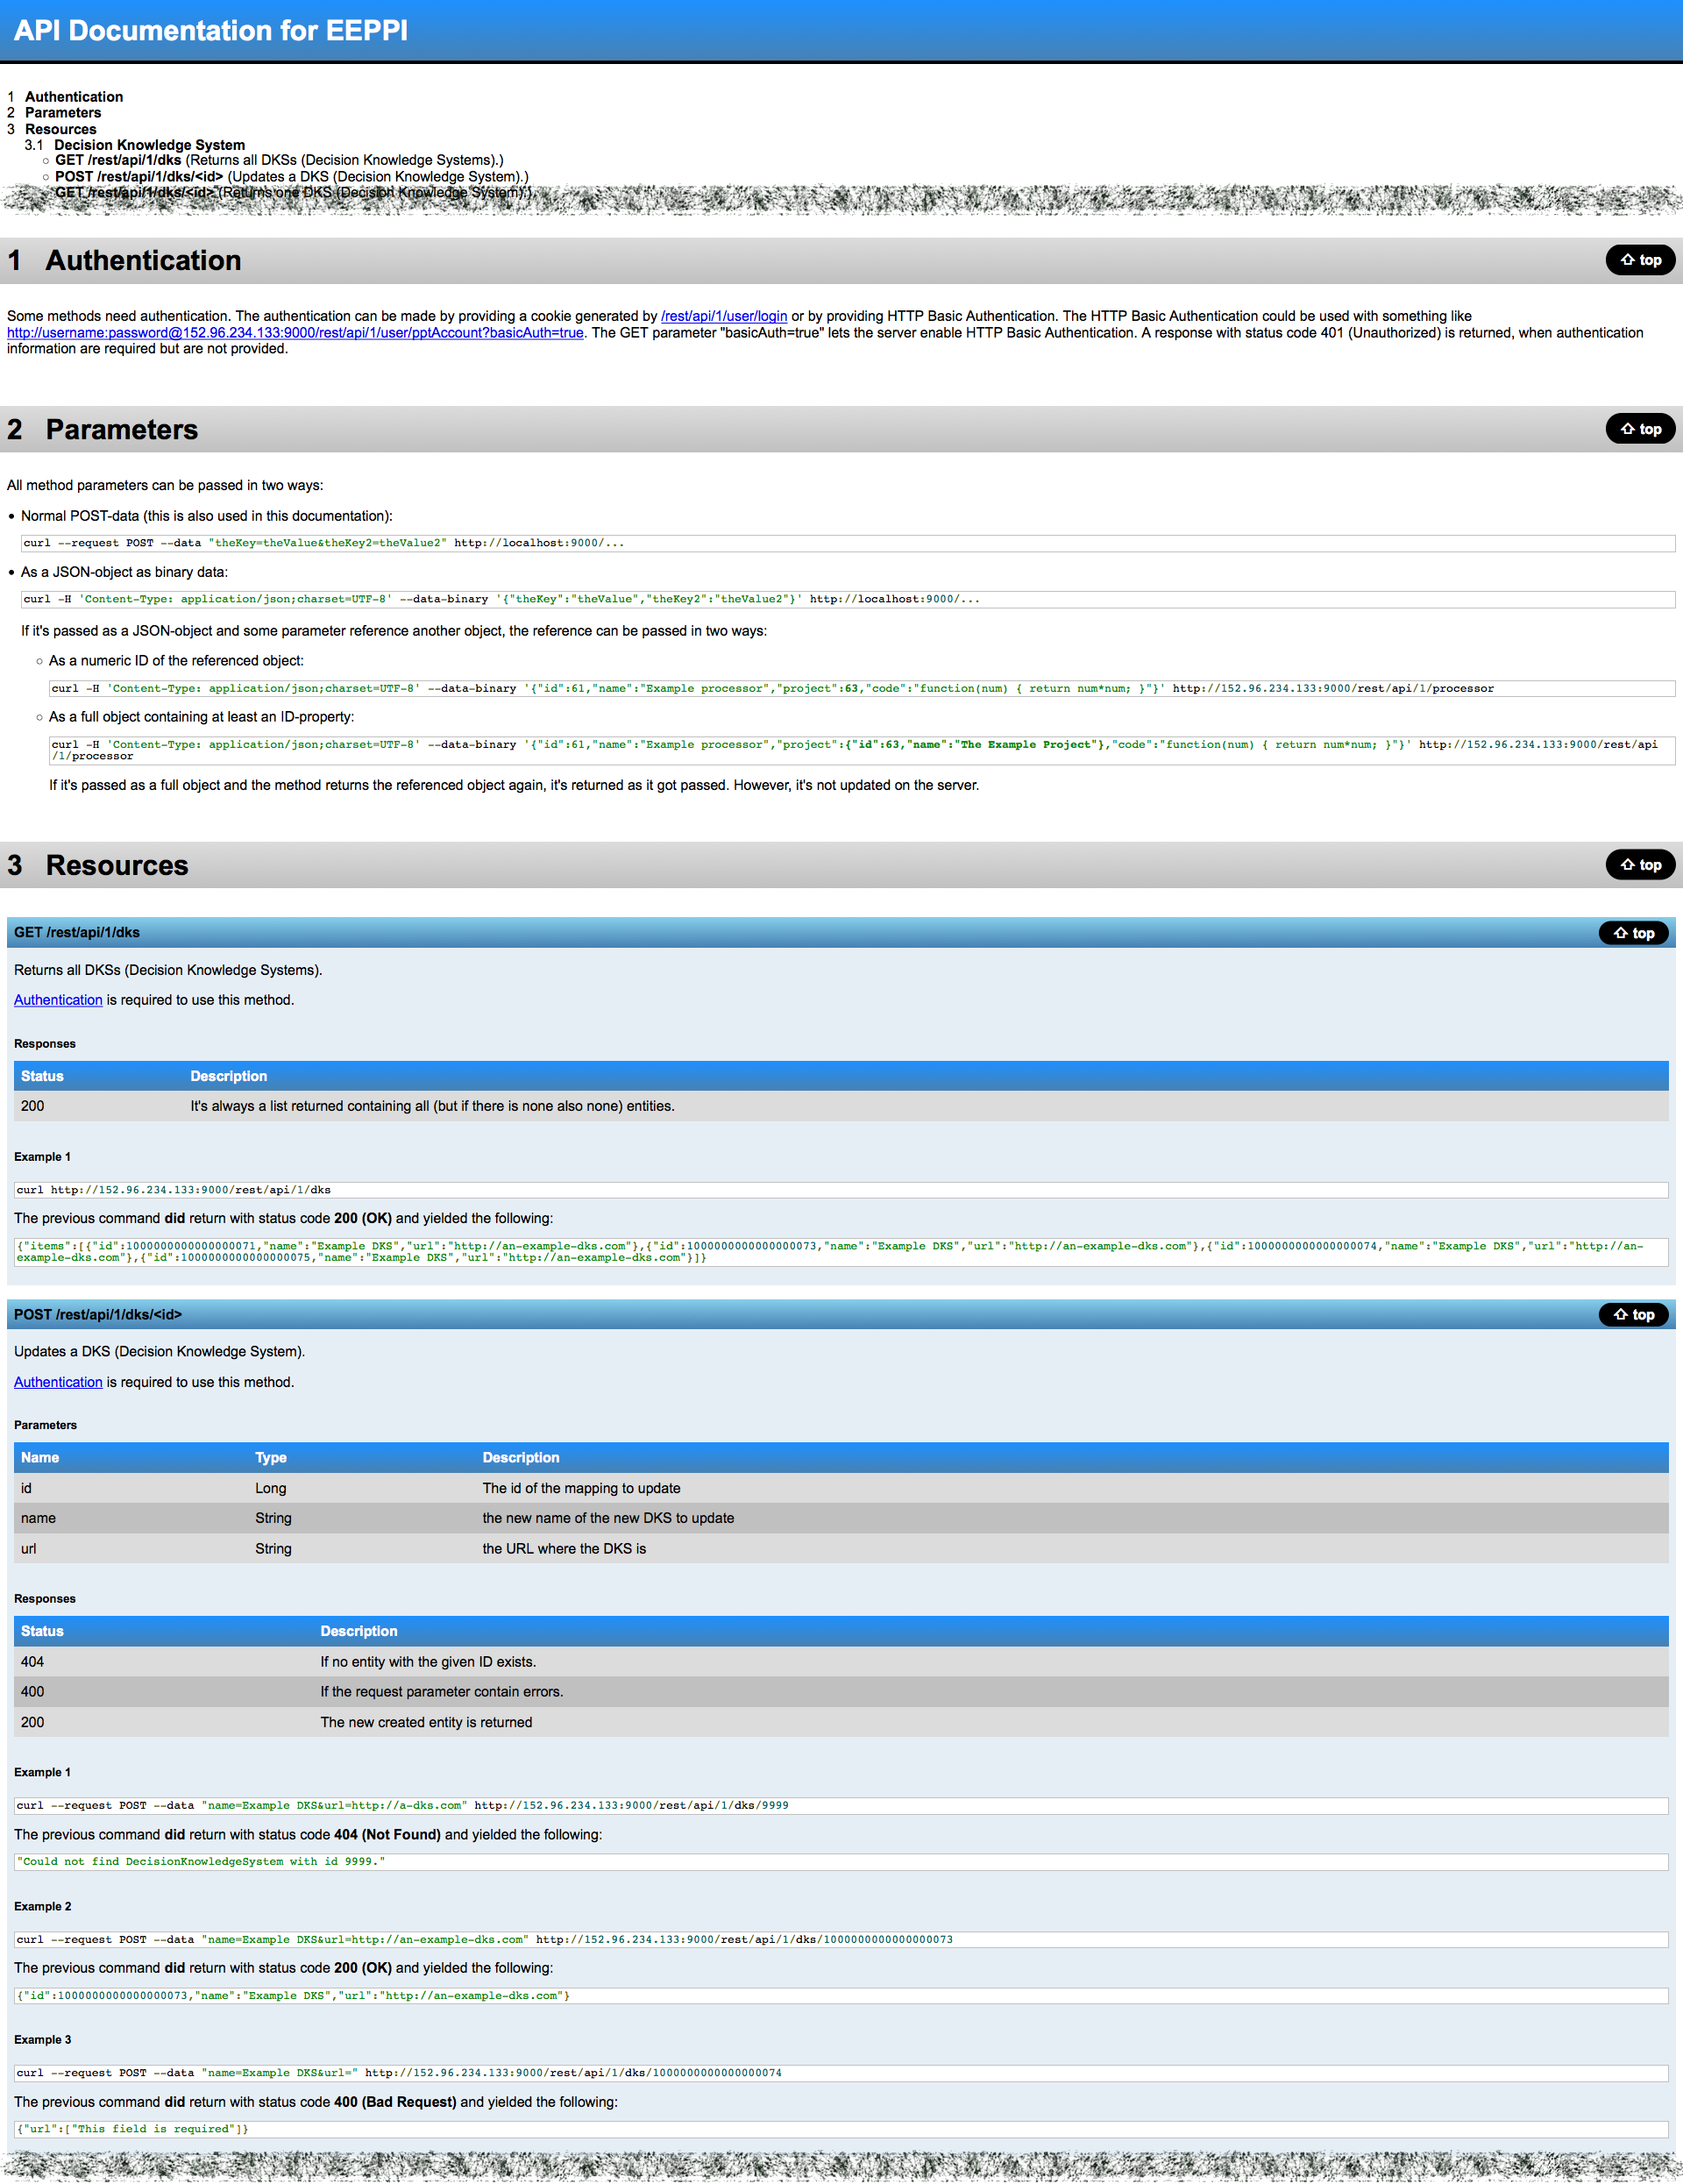
\includegraphics[width=\textwidth]{codeDocumentation/media/img/apiDocumentation.png}
		\centering
		\caption{Auszug aus der API-Dokumentation}
		\label{fig:apiScreenshot}
	\end{figure}
